\documentclass[11pt,a4paper]{amsart}
\usepackage[a4paper,margin=1in]{geometry}
\usepackage[T1]{fontenc}
\usepackage{lmodern}
\usepackage{amsmath,amssymb,mathtools}
\usepackage{microtype}
\usepackage{tikz}
\usepackage{xcolor}
\usepackage{hyperref}
\definecolor{linkblue}{RGB}{35,72,139}
\hypersetup{colorlinks=true,linkcolor=linkblue,citecolor=linkblue,urlcolor=linkblue,
  pdftitle={Uniform exclusion of Landau-Siegel zeros},pdfauthor={OpenAI}}
\pdftrailerid{}
\pdfinfoomitdate=1
\pdfsuppressptexinfo=15
\newtheorem{theorem}{Theorem}
\newtheorem{lemma}[theorem]{Lemma}
\newtheorem{corollary}[theorem]{Corollary}
\newtheorem{proposition}[theorem]{Proposition}
\theoremstyle{remark}
\newtheorem{remark}[theorem]{Remark}
\newcommand{\Q}{\mathbb Q}
\newcommand{\Z}{\mathbb Z}
\newcommand{\C}{\mathbb C}
\newcommand{\R}{\mathbb R}
\newcommand{\N}{\mathbb Z_{\ge0}}
\newcommand{\cR}{\mathcal R}
\newcommand{\cP}{\mathcal P}
\newcommand{\cK}{\mathcal K}
\DeclareMathOperator{\Gal}{Gal}
\DeclareMathOperator{\Nm}{N}
\DeclareMathOperator{\conv}{conv}
\numberwithin{equation}{section}
\title{Uniform exclusion of Landau--Siegel zeros}
\author{OpenAI}
\date{October 1, 2026}
\subjclass[2020]{Primary 11M20; Secondary 11J81, 14L17.}
\keywords{Dirichlet L-functions, Landau--Siegel zeros, polynomial interpolation,
interpolation determinants}
\begin{document}
\begin{abstract}
We prove the uniform exclusion of Landau--Siegel zeros. There is an
absolute constant $c>0$ such that every real zero $\beta\in(0,1)$ of
every primitive nonprincipal real Dirichlet $L$-function of conductor
$q\ge3$ satisfies $(1-\beta)\log q\ge c$.
\end{abstract}
\maketitle

\section{Introduction}\label{sec:intro}

For a primitive Dirichlet character $\chi$ of conductor $q$, let
\[
 L(s,\chi)=\sum_{n\ge1}\frac{\chi(n)}{n^s}
 \qquad(\operatorname{Re}s>1),
\]
and use its analytic continuation elsewhere. For an absolute constant
$c_1>0$, the classical region
\[
 \operatorname{Re}s\ge1-\frac{c_1}{\log(q(|\operatorname{Im}s|+2))}
\]
is zero-free except for a possible simple real zero attached to a real
character \cite[Section~14]{Davenport}. Excluding this possibility
uniformly is the Landau--Siegel zero problem. We prove its logarithmic
formulation.

\begin{theorem}\label{thm:main}
There is an absolute constant $c>0$ such that every real zero
$\beta\in(0,1)$ of every primitive nonprincipal real Dirichlet
$L$-function of conductor $q\ge3$ satisfies
\begin{equation}\label{eq:main}
 (1-\beta)\log q\ge c.
\end{equation}
\end{theorem}

Possible exceptional zeros obstruct uniform estimates for primes in
arithmetic progressions. They also affect the study of quadratic
class numbers through the values $L(1,\chi)$ in Dirichlet's
class-number formula. Siegel's theorem of 1935 gives
$L(1,\chi)\gg_\varepsilon q^{-\varepsilon}$ for every
$\varepsilon>0$, with an ineffective constant \cite{Siegel,Davenport}.
This estimate leaves open the possibility of a sequence of real zeros
with $(1-\beta)\log q\to0$. More uniformly across characters,
Page's theorem gives an absolute constant $c_2>0$ such that, for every
$Q\ge3$, at most one primitive real character of conductor at most $Q$
has a real zero in $(1-c_2/\log Q,1)$ \cite{Page}. The common window
depends on $Q$, not on each character's own conductor.
The Deuring--Heilbronn phenomenon, developed quantitatively by
Linnik and Heath-Brown, forces
other zeros away from $1$ \cite{Linnik,HeathBrown}; see Benli,
Goel, Twiss, and Zaman \cite{BGTZ} for a recent explicit form.
Friedlander and Iwaniec
\cite{FI} discuss the logarithmic zero-gap conjecture and its relation
to lower bounds for $L(1,\chi)$.

\subsection*{The argument}
The analytic starting point is that a zero with
$(1-\beta)\log q$ small forces a shortage of primes with $\chi(p)=1$;
compare \cite[Section~5]{FI}. Consequently, primes with $\chi(p)=-1$
carry enough logarithmic mass for the determinant comparison. We give the
short logarithmic-derivative proof in Section~\ref{sec:analytic}.

The remaining argument is algebraic. Associate to $\chi$ a quadratic
field $\Q(\sqrt d)$ and adjoin $\sqrt2$. Except for one fixed quadratic
field, this gives a biquadratic field $K=\Q(a,b)$, with
$a^2=d$ and $b^2=2$. Let $\sigma$ change the sign of $a$ and let
$\tau$ change the sign of $b$. For
$n=(n_1,n_2,n_3,n_4)\in\{0,\ldots,N-1\}^4$, put
\[
 \theta_n=n_1+n_2a+n_3b+n_4ab.
\]
We form rows indexed by triples $\alpha\in\N^3$ whose entries are
\[
 \theta_n^{\alpha_1}\sigma(\theta_n)^{\alpha_2}
                  \sigma\tau(\theta_n)^{\alpha_3}.
\]
There are $N^4$ columns. The interpolation estimate supplies enough
independent rows to form a nonzero square determinant at the natural
degree scale $U=N^{4/3}$, for which
$U^3=N^4$. To favor the first exponent, we order the rows by
$\alpha_1+H\alpha_2+H\alpha_3$ and retain a row exactly when it
increases the span of its predecessors. Here the integer $H$ will
be large and fixed. Summed over the retained rows, the last two
exponents account for an arbitrarily small fraction of the total degree.

At an odd prime $p\nmid q$ with $\chi(p)=-1$, taking $p$-th powers
modulo $p$ sends $\theta_n$ to either $\sigma(\theta_n)$ or
$\sigma\tau(\theta_n)$. When $p>H$, replacing a block of $p$ first
factors by the corresponding conjugate strictly lowers the row
weight. Subtraction therefore preserves the determinant and extracts
powers of $p$ from the rows. Primes up to $U$ contribute the leading
factor $\log U$ to the divisibility bound, whereas the evaluation
points contribute $\log N=\tfrac34\log U$ to the size bound.
This strict difference drives the contradiction. Taking $N$ to be
a sufficiently large fixed power of $q$ controls the additional
$\log q$ term in the size bound.
Section~\ref{sec:determinant} constructs the rows,
Section~\ref{sec:comparison} proves the two bounds, and
Section~\ref{sec:conclusion} makes the parameter choices.

\subsection*{Interpolation and arithmetic context}
The reusable algebraic input is Lemma~\ref{lem:interpolation}, proved
in Section~\ref{sec:interpolation}. It bounds the separate degrees
needed to interpolate on a linear image of an integer box in $\C^4$.
Its hypothesis is that the kernel is spanned by a vector whose
coordinates are linearly independent over $\Q$. The estimate is uniform in the linear
map and in the choice of coordinates on the three-dimensional image.
This allows the interpolation box to have an arbitrarily large fixed
aspect ratio without introducing a constant depending on the field.
The proof uses a dimension count, a nearest-point argument for an
integer polytope, and Lagrange interpolation on a supporting face.

General multiplicity estimates on commutative algebraic groups are
developed in \cite{Philippon}; rectangular derivative conditions
and interpolation duality appear in
\cite[Theorem~1.1 and Lemma~1.3]{Fischler}. The estimate proved here
makes the coefficient and coordinate uniformity explicit. The final
comparison belongs to the interpolation-determinant method described
by Laurent \cite[Section~6]{Laurent}. Bost's arithmetic algebraicity
criteria use spaces of derivations closed under $p$-fold composition
at almost all prime ideals \cite[Theorems~2.1 and 2.3]{Bost}.
In the torus interpretation recalled in Section~\ref{sec:interpolation},
our argument controls this operation on one distinguished derivation
at selected primes and uses it directly for determinant divisibility,
rather than applying an algebraicity criterion. All algebraic estimates
used in the proof are established below.

All logarithms are natural. Constants
implicit in $O(\cdot)$ and $\ll$ are absolute unless a dependence is
specified. All vector-space spans are over the indicated field, and
we use $z^0=1$, including when $z=0$.

\section{The prime bias forced by a real zero}\label{sec:analytic}

We first record the prime-sum estimate that will be compared with the
determinant bound. Let $\chi$ be primitive, nonprincipal, and real of
conductor $q\ge3$, and let $\beta\in(0,1)$ be a real zero. Write
\[
 \ell=\log q,\qquad \delta=(1-\beta)\ell.
\]

\begin{lemma}\label{lem:primebias}
For $X\ge3$,
\begin{equation}\label{eq:primebias}
 \sum_{\substack{p\le X\\\chi(p)=1}}\frac{\log p}{p}
 \ll \ell+\frac{\delta(\log X)^2}{\ell}.
\end{equation}
Consequently, for each integer $H\ge2$,
\begin{equation}\label{eq:mass}
 \sum_{\substack{H<p\le X\\p\nmid2q\\\chi(p)=-1}}
     \frac{\log p}{p}
 \ge \log X-C\ell-C\frac{\delta(\log X)^2}{\ell}-C_H,
\end{equation}
where $C$ is absolute and $C_H$ depends only on $H$.
\end{lemma}

\begin{proof}
Put $\varepsilon=(1-\chi(-1))/2$. For the completed function
\[
 \Lambda_\chi(s)=
 (q/\pi)^{(s+\varepsilon)/2}
 \Gamma\bigl((s+\varepsilon)/2\bigr)L(s,\chi),
\]
the Hadamard product and functional equation give, for real $s>1$,
\begin{equation}\label{eq:hadamard}
 -\frac{L'}{L}(s,\chi)
 =\frac12\log\frac q\pi
  +\frac12\frac{\Gamma'}{\Gamma}
        \bigl((s+\varepsilon)/2\bigr)
  -\sum_\rho\operatorname{Re}\frac1{s-\rho}.
\end{equation}
Here $\rho$ runs over the nontrivial zeros with multiplicity. The sum
of real parts converges, and each term is nonnegative. This is the
standard logarithmic-derivative identity; see
\cite[Sections~12 and 14]{Davenport}. The functional equation cancels
the real constant from the Hadamard product. For $1<s\le2$, the gamma
term is bounded for both parities. Keeping only the term for $\beta$
and using $-\zeta'/\zeta(s)=1/(s-1)+O(1)$ gives
\begin{equation}\label{eq:logderivative}
 -\frac{\zeta'}{\zeta}(s)-\frac{L'}{L}(s,\chi)
 \le C\ell+\frac1{s-1}-\frac1{s-\beta}.
\end{equation}

Take $s=1+1/\log X$, which lies in $(1,2)$ for $X\ge3$.
Writing $\Lambda(n)$ for the von Mangoldt function, the Euler
products give the nonnegative series
\[
 -\frac{\zeta'}{\zeta}(s)-\frac{L'}{L}(s,\chi)
 =\sum_{n\ge1}\frac{\Lambda(n)(1+\chi(n))}{n^s}
 \ge\frac2e\sum_{\substack{p\le X\\\chi(p)=1}}\frac{\log p}{p}.
\]
Also,
\[
 \frac1{s-1}-\frac1{s-\beta}
 =\frac{1-\beta}{(s-1)(s-\beta)}
 \le(1-\beta)(\log X)^2.
\]
This proves \eqref{eq:primebias}. To obtain \eqref{eq:mass}, use
Mertens' estimate and the elementary bound for primes dividing $q$:
\[
 \sum_{p\le X}\frac{\log p}{p}=\log X+O(1),
 \qquad \sum_{p\mid q}\frac{\log p}{p}\le\log q.
\]
Removing primes at most $H$ costs a constant depending only on $H$.
\end{proof}

\section{Interpolation on a projected integer box}\label{sec:interpolation}

The purpose of this section is to obtain a nonzero evaluation
determinant using monomials whose separate degrees may be very
different. No arithmetic estimates enter the interpolation lemma.

\begin{lemma}\label{lem:interpolation}
Let $A:\C^4\to\C^3$ be a surjective linear map, with $\ker A=\C c$, where the
four coordinates of $c$ are linearly independent over $\Q$.
Let $N\ge1$ and $t_1,t_2,t_3$ be integers satisfying
\begin{equation}\label{eq:budget}
 t_j\ge3(N-1)\quad(1\le j\le3),\qquad
 \prod_{j=1}^3\bigl(t_j-3(N-1)+1\bigr)>(4N-3)^4.
\end{equation}
Set $E_N=\{0,\ldots,N-1\}^4$ and
\[
 \cP_t=\{B\in\C[z_1,z_2,z_3]:\deg_{z_j}B\le t_j
                                      \text{ for }1\le j\le3\}.
\]
Then the evaluation map $B\mapsto(B(An))_{n\in E_N}$ from
$\cP_t$ to $\C^{E_N}$ is surjective.
\end{lemma}

\begin{proof}
Suppose the evaluation map is not surjective. There are complex
numbers $v_n$, not all zero, such that
\begin{equation}\label{eq:moments}
 \sum_{n\in E_N}v_nB(An)=0\qquad(B\in\cP_t).
\end{equation}
Let $S=\{n:v_n\ne0\}$ and $P=\conv(S)\subset\R^4$.
We construct the test polynomial as a product. A translated
polynomial will vanish at $An$ for every $n\in S$ outside one
supporting face of $P$. A second polynomial will select a single
vertex on that face, with total degree at most $3(N-1)$.

Put $\cK=4P$. For $b_j=t_j-3(N-1)$, the polynomials of separate degrees
at most $b_j$ form a vector space of dimension $\prod_j(b_j+1)$.
Since
\[
 \cK\subset[0,4(N-1)]^4,\qquad
 \#(\cK\cap\Z^4)\le(4N-3)^4<\prod_j(b_j+1),
\]
there is a nonzero polynomial $R$ with $\deg_{z_j}R\le b_j$ and
\begin{equation}\label{eq:zeros}
 R(Am)=0\qquad(m\in\cK\cap\Z^4).
\end{equation}

\smallskip\noindent
\emph{A supporting face.}
The polynomial $R\circ A$ is nonzero because $A$ is surjective.
A nonzero polynomial on $\C^4$ cannot vanish on all of $\Z^4$:
this follows by applying the one-variable root bound successively
to its four coordinates. Choose $m\in\Z^4$ with $R(Am)\ne0$ whose
distance to $\cK$ is least. Such a minimum exists because bounded
neighborhoods of the compact set $\cK$ contain finitely many lattice
points. Let $y\in\cK$ be nearest to $m$ and set $h=m-y$.
By \eqref{eq:zeros}, $h\ne0$.

The nearest-point inequality
$h\cdot(x-y)\le0$ for $x\in\cK$ shows that $y/4$ belongs to
the supporting face
\[
 G=\{v\in P:h\cdot v=\max_{w\in P}h\cdot w\}.
\]
This face has dimension at most three: if $P$ is four-dimensional
then $G$ is proper, and otherwise $\dim G\le\dim P\le3$.
Removing affine dependencies from a convex combination expresses
$y/4$ as a combination of at most four vertices of $G$. One
coefficient is at least $1/4$. Choosing its vertex $u$ gives
\begin{equation}\label{eq:vertex}
 u\in S\cap G,\qquad y-u\in3P.
\end{equation}
Indeed, subtracting $u$ from four times that convex combination
leaves nonnegative coefficients with sum three.

For $n\in S\setminus G$, define
\[
 y'=y+n-u\in4P,\qquad m'=m+n-u=y'+h.
\]
The inclusion follows from \eqref{eq:vertex}. Since
$h\cdot(u-n)>0$, for sufficiently small $\eta>0$ the point
$y'+\eta(y-y')\in\cK$ satisfies
\begin{equation}\label{eq:distance}
 \bigl\|m'-[y'+\eta(y-y')]\bigr\|^2
 =\|h-\eta(u-n)\|^2<\|h\|^2.
\end{equation}
Thus $m'$ is closer to $\cK$ than $m$ is. By the choice of $m$,
\begin{equation}\label{eq:offface}
 R\bigl(A(m+n-u)\bigr)=0\qquad(n\in S\setminus G).
\end{equation}
Figure~\ref{fig:nearest} illustrates the strict decrease in distance.

\begin{figure}[ht]
\centering
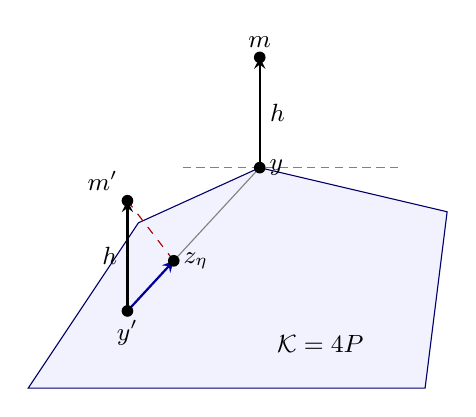
\begin{tikzpicture}[scale=1.4,>=stealth,font=\small]
 \filldraw[fill=blue!5,draw=blue!40!black]
 (0,0)--(3.6,0)--(3.8,1.6)--(2.1,2)--(1,1.5)--cycle;
 \node at (2.65,.4) {$\cK=4P$};
 \draw[densely dashed,gray] (1.4,2)--(3.4,2);
 \coordinate (y) at (2.1,2);
 \coordinate (m) at (2.1,3);
 \coordinate (yp) at (.9,.7);
 \coordinate (mp) at (.9,1.7);
 \coordinate (z) at (1.32,1.155);
 \draw[->,thick] (y)--node[right] {$h$}(m);
 \draw[->,thick] (yp)--node[left] {$h$}(mp);
 \draw[gray] (yp)--(y);
 \draw[->,thick,blue!60!black] (yp)--(z);
 \draw[dashed,red!65!black] (mp)--(z);
 \fill (y) circle (1.5pt) node[right] {$y$};
 \fill (m) circle (1.5pt) node[above] {$m$};
 \fill (yp) circle (1.5pt) node[below] {$y'$};
 \fill (mp) circle (1.5pt) node[above left] {$m'$};
 \fill (z) circle (1.5pt) node[right] {$z_\eta$};
\end{tikzpicture}
\caption{Schematic of \eqref{eq:distance}. Both $y$ and $y'$ lie in
$\cK$, and $m-y=m'-y'=h$. Moving to $z_\eta=y'+\eta(y-y')$ decreases the
distance to $m'$ because $h\cdot(y-y')>0$. The dashed red segment is
shorter than $\|h\|$; the argument takes place in $\R^4$.}
\label{fig:nearest}
\end{figure}

\smallskip\noindent
\emph{Interpolation on the face.}
The integer vertices of $G$ span an affine space of dimension at most
three. Solving their affine linear equations over $\Q$ and clearing
denominators gives a hyperplane
\[
 \mathcal H=\{v\in\C^4:r\cdot v=k\},
 \qquad 0\ne r\in\Z^4,\quad k\in\Z,
\]
containing $G$. Rational independence gives $r\cdot c\ne0$.
The restriction $A|_{\mathcal H}$ is therefore an affine bijection
onto $\C^3$: each affine line parallel to $\ker A$ meets
$\mathcal H$ exactly once.

Choose $i_0$ with $r_{i_0}\ne0$. The other three coordinates
determine a point of $\mathcal H$. Let $\lambda_i(z)$, for
$i\ne i_0$, be those affine coordinate functions of
$(A|_{\mathcal H})^{-1}(z)$. Thus $\lambda_i(An)=n_i$ for
$n\in\mathcal H$. The Lagrange polynomial
\[
 Q(z)=\prod_{i\ne i_0}\ \prod_{\substack{0\le a<N\\a\ne u_i}}
             \frac{\lambda_i(z)-a}{u_i-a}
\]
has total degree at most $3(N-1)$ and satisfies
\[
 Q(An)=\begin{cases}1,&n=u,\\0,&n\in(S\cap G)\setminus\{u\}.
 \end{cases}
\]
The denominators are nonzero integers; empty products are $1$.

Now set $B(z)=Q(z)R(z+A(m-u))$. Translation preserves each separate
degree of $R$, and the total degree bound on $Q$ bounds each of its
separate degrees. Hence $B\in\cP_t$. Equation~\eqref{eq:offface}
eliminates the terms off $G$, and $Q$ eliminates all remaining terms
except the one at $u$. Substitution in \eqref{eq:moments} gives
the contradiction
\[
 0=\sum_{n\in S}v_nQ(An)R\bigl(A(m+n-u)\bigr)
   =v_uR(Am)\ne0.\qedhere
\]
\end{proof}

\begin{corollary}\label{cor:rectangle}
Let $A$ satisfy the hypotheses of Lemma~\ref{lem:interpolation}.
For integers $1\le H\le N$, set
\[
 U=N^{4/3},\qquad T_1=32H^{2/3}U,
 \qquad T_2=T_3=32H^{-1/3}U.
\]
The rows $((An)_1^{\alpha_1}(An)_2^{\alpha_2}(An)_3^{\alpha_3})_{n\in E_N}$,
with $\alpha\in\N^3$ and $\alpha_j\le T_j$, span $\C^{E_N}$.
The constant $32$ is independent of $A$ and $H$.
\end{corollary}

\begin{proof}
Put $t_j=\lfloor T_j\rfloor$. Since $H\le N$, every $T_j\ge32N$,
and $T_1T_2T_3=32^3N^4$. In particular $t_j\ge3(N-1)$, and
\[
 \prod_{j=1}^3\bigl(t_j-3(N-1)+1\bigr)
 >\prod_{j=1}^3\bigl(T_j-3(N-1)\bigr)
 \ge\frac{T_1T_2T_3}{8}
 =4096N^4>(4N-3)^4.
\]
Apply Lemma~\ref{lem:interpolation} to the monomial basis of $\cP_t$.
\end{proof}

\begin{remark}
The connection with multiplicity estimates is immediate. On
$(\C^\times)^4$, write $D_j=\sum_i A_{ji}x_i\partial/\partial x_i$.
For $x^n=x_1^{n_1}\cdots x_4^{n_4}$,
$(D_1^{\alpha_1}D_2^{\alpha_2}D_3^{\alpha_3}x^n)(1,1,1,1)=(An)^\alpha$.
Thus Corollary~\ref{cor:rectangle} is a rectangular multiplicity
estimate. This interpolation viewpoint is standard in the subject;
compare \cite[Section~1]{Fischler}. We use the evaluation rows
directly in what follows.
\end{remark}

\section{A weighted determinant of conjugates}\label{sec:determinant}

We now construct a nonzero determinant for which most of the total
exponent lies in the first coordinate. This is the coordinate to
which the prime congruence will apply.

A primitive nonprincipal real character $\chi$ corresponds to a
fundamental discriminant $D$ with $|D|=q$. Write
$\Q(\sqrt D)=\Q(\sqrt d)$ with $d$ squarefree. Then
$|d|\le q$ and, for odd $p\nmid q$,
$\chi(p)=(d/p)$, the Legendre symbol; see \cite{Davenport}.
Temporarily exclude $d=2$ and put
\[
 a=\sqrt d,\qquad b=\sqrt2,\qquad K=\Q(a,b),\qquad
 \cR=\Z[a,b].
\]
Since $\chi$ is nonprincipal, $d\ne1$, so $[K:\Q]=4$.
Every element of $\cR$ has a unique expression
$z_1+z_2a+z_3b+z_4ab$ with $z_i\in\Z$.
The automorphisms $\sigma(a)=-a$, $\sigma(b)=b$ and
$\tau(a)=a$, $\tau(b)=-b$ generate $\Gal(K/\Q)$.

For integers $1\le H\le N$, retain the notation $U=N^{4/3}$ and set
$M=N^4=U^3$. For $n\in E_N$ define
$\theta_n=n_1+n_2a+n_3b+n_4ab$. The map
\begin{equation}\label{eq:A}
 A=\begin{pmatrix}
 1&a&b&ab\\1&-a&b&-ab\\1&-a&-b&ab
 \end{pmatrix}
 \quad\text{satisfies}\quad
 An=(\theta_n,\sigma(\theta_n),\sigma\tau(\theta_n)).
\end{equation}
It has rank three and
\[
 \ker A=\C(ab,b,-a,-1).
\]
For example, the minor in the first three columns is $4ab\ne0$,
and multiplication verifies the displayed kernel. Its four
coordinates are linearly independent over $\Q$ because
$1,a,b,ab$ are a $\Q$-basis of $K$. Thus
Corollary~\ref{cor:rectangle} applies.

For $\alpha\in\N^3$, write
\begin{equation}\label{eq:rows}
 R_\alpha=
 \bigl(\theta_n^{\alpha_1}\sigma(\theta_n)^{\alpha_2}
                   \sigma\tau(\theta_n)^{\alpha_3}\bigr)_{n\in E_N}.
\end{equation}
Fix an order of the columns. Order all indices in $\N^3$ by increasing
$w(\alpha)=\alpha_1+H\alpha_2+H\alpha_3$, with any fixed rule to
break ties. Retain a row precisely when it increases the span of
the earlier rows over $K$. Rank is unchanged on extending scalars
from $K$ to $\C$, so Corollary~\ref{cor:rectangle} guarantees $M$
retained rows. Every row in that corollary has weight at most
$T_1+HT_2+HT_3=96H^{2/3}U$. Therefore all retained rows have weight
at most this bound.

Let $\cP$ be the set of retained indices, in their retained order,
and put
\begin{equation}\label{eq:det}
 \Delta=\det(R_\alpha)_{\alpha\in\cP}\in\cR\setminus\{0\},
 \qquad S_1=\sum_{\alpha\in\cP}\alpha_1,
 \qquad S_2=\sum_{\alpha\in\cP}(\alpha_2+\alpha_3).
\end{equation}
Only the surjectivity conclusion of Corollary~\ref{cor:rectangle}
enters the selection of these rows. The coefficients of the auxiliary
polynomials used to prove it may depend on $A$, but they do not enter
$\Delta$, which is formed from the original monomial rows. Thus no
bound on those coefficients is needed for the size estimate below.
This is the interpolation-determinant construction, with a weighted row order; compare
\cite[Section~6]{Laurent}.

\begin{lemma}\label{lem:exponents}
There are absolute constants $c_0,C_0>0$ such that for every fixed
integer $H\ge1$ and all sufficiently large $N$ in terms of $H$ alone,
\begin{equation}\label{eq:exponents}
 S_1\ge c_0MH^{2/3}U,\qquad S_2\le C_0MH^{-1/3}U.
\end{equation}
In particular, $S_2/S_1\le(C_0/c_0)/H$.
\end{lemma}

\begin{proof}
The weight bound gives
$\alpha_2,\alpha_3\le B:=96H^{-1/3}U$ for every retained index.
Thus $S_2\le192MH^{-1/3}U$. For each fixed value of $\alpha_1$,
there are at most
\[
 Q_0=(\lfloor B\rfloor+1)^2\le97^2H^{-2/3}U^2
\]
retained indices; here $H^{-1/3}U\ge1$ follows from $N\ge H$.
List the first coordinates in increasing order as
$b_1,\ldots,b_M$. Then $b_i\ge\lfloor(i-1)/Q_0\rfloor$.
Writing $M=kQ_0+r$, $0\le r<Q_0$, gives
\[
 S_1\ge Q_0\frac{k(k-1)}2+kr
 \ge\frac{M^2}{2Q_0}-\frac M2.
\]
The last inequality has difference $r(Q_0-r)/(2Q_0)\ge0$.
For fixed $H$, the condition $M\ge2Q_0$ holds whenever
$H^{2/3}N^{4/3}\ge2\cdot97^2$. Thus, uniformly in the field,
\[
 S_1\ge\frac{M^2}{4Q_0}
 \ge\frac{MH^{2/3}U}{4\cdot97^2}.
\]
We may take $c_0=(4\cdot97^2)^{-1}$ and $C_0=192$.
\end{proof}

\section{Two bounds for the determinant}\label{sec:comparison}

For $z\in K$, define
$\Nm(z)=z\sigma(z)\tau(z)\sigma\tau(z)$.
If $z\in\cR$, then $\Nm(z)\in\Z$: its product belongs to
$\cR$ and is fixed by both $\sigma$ and $\tau$, so only its
integer constant coefficient remains. In particular
$\Nm(\Delta)$ is a nonzero integer. We bound its absolute value
from above at the complex embeddings and from below by divisibility.

\subsection*{The Archimedean bound}
For every embedding $\nu:K\hookrightarrow\C$ and every $n\in E_N$,
\[
 |\nu(\theta_n)|
 \le(N-1)(1+\sqrt{|d|})(1+\sqrt2)
 \le8N\sqrt q.
\]
This estimate is valid for either sign of $d$. Each row indexed by
$\alpha$ has Euclidean norm at most
$\sqrt M(8N\sqrt q)^{\alpha_1+\alpha_2+\alpha_3}$ at every embedding.
Hadamard's inequality and the four embeddings give
\begin{equation}\label{eq:upper}
 \frac14\log|\Nm(\Delta)|
 \le\frac M2\log M+
 (S_1+S_2)\bigl(\log N+\tfrac12\ell+\log8\bigr).
\end{equation}

\subsection*{The prime divisibility}
Call a prime $p$ admissible if
$p>H$, $p\nmid2q$, and $\chi(p)=-1$. Euler's criterion gives
in $\cR/p\cR$
\[
 a^p=a\,d^{(p-1)/2}\equiv-a,
 \qquad b^p=b\,2^{(p-1)/2}\equiv(2/p)b.
\]
The $p$-th-power map is a ring homomorphism in characteristic $p$,
and integer coefficients are fixed by it. Consequently
\begin{equation}\label{eq:frobenius}
 \theta^p\equiv g_p(\theta)\pmod{p\cR}
 \quad(\theta\in\cR),\qquad
 g_p=\begin{cases}\sigma,&(2/p)=1,\\
                   \sigma\tau,&(2/p)=-1.
       \end{cases}
\end{equation}
This is the Frobenius relation in the ring $\cR$.

\begin{lemma}\label{lem:divisibility}
For every admissible prime $p$,
\begin{equation}\label{eq:divisibility}
 \Delta\in p^{E_p}\cR,
 \qquad E_p=\sum_{\alpha\in\cP}\left\lfloor\frac{\alpha_1}{p}\right\rfloor.
\end{equation}
\end{lemma}

\begin{proof}
Let $j=2$ or $3$ according as $g_p=\sigma$ or $\sigma\tau$.
For a retained index $\alpha$, write $\alpha_1=pk+r$ with
$0\le r<p$. In \eqref{eq:rows}, replace the first factor by
\[
 \theta_n^r\bigl(\theta_n^p-g_p(\theta_n)\bigr)^k
\]
and leave the other two factors unchanged. Denote the resulting row
by $\widetilde R_\alpha$. Expansion yields the exact identity
\begin{equation}\label{eq:replacement}
 \widetilde R_\alpha
 =R_\alpha+\sum_{m=1}^k(-1)^m\binom{k}{m}
                       R_{\alpha-pm e_1+me_j},
\end{equation}
where $e_1,e_2,e_3$ are the standard coordinate vectors.
Every row on the right after $R_\alpha$ has smaller weight, since
its weight is $w(\alpha)-m(p-H)$.

By the greedy selection rule, every earlier row lies in the
$K$-span of the earlier retained rows. Thus the matrix of replacement
rows equals $L$ times the matrix of retained rows, where $L$ is lower
triangular over $K$ with diagonal entries $1$. In particular,
\begin{equation}\label{eq:det-preserved}
 \det(\widetilde R_\alpha)_{\alpha\in\cP}=\Delta.
\end{equation}
On the other hand, \eqref{eq:frobenius} shows that every entry of
$\widetilde R_\alpha$ belongs to $p^k\cR$. Dividing its entries
by $p^k$ leaves a matrix over $\cR$. Factoring these powers from
\eqref{eq:det-preserved} proves \eqref{eq:divisibility}.
The equality of determinants is over $K$; the divisibility follows
from the replacement entries themselves, so no integrality of $L$
is required.
\end{proof}

Taking norms in \eqref{eq:divisibility} gives
$p^{4E_p}\mid\Nm(\Delta)$. Since the norm is a nonzero integer,
distinct admissible primes may be combined. Therefore
\begin{align}
 \frac14\log|\Nm(\Delta)|
 &\ge\sum_{\substack{p\le U\\p\ \mathrm{admissible}}}E_p\log p\notag\\
 &\ge S_1\sum_{\substack{p\le U\\p\ \mathrm{admissible}}}
                          \frac{\log p}{p}
       -M\sum_{p\le U}\log p.\label{eq:lower-primes}
\end{align}
The second inequality uses $\lfloor x\rfloor\ge x-1$ in each row.
Chebyshev's bound $\sum_{p\le U}\log p\ll U$ and
Lemma~\ref{lem:primebias} now give, when $U\ge3$ and $H\ge2$,
\begin{equation}\label{eq:lower}
 \frac14\log|\Nm(\Delta)|
 \ge S_1\left(\log U-C\ell
       -C\frac{\delta(\log U)^2}{\ell}-C_H\right)-CMU.
\end{equation}
The leading term here is $S_1\log U$. In \eqref{eq:upper}, the
corresponding term is $(S_1+S_2)\log N$, and
$\log N=\tfrac34\log U$. The weight $H$ makes $S_2/S_1$ small
enough to preserve this difference.

\section{Completion of the proof}\label{sec:conclusion}

Suppose Theorem~\ref{thm:main} is false. Then there is a sequence
of primitive nonprincipal real characters and real zeros with
\begin{equation}\label{eq:sequence}
 q\longrightarrow\infty,\qquad
 \delta=(1-\beta)\log q\longrightarrow0.
\end{equation}
To justify $q\to\infty$, there are only finitely many characters
of bounded conductor, and for each of them $L(1,\chi)\ne0$.
Analyticity therefore prevents zeros from accumulating at $1$.
Passing to a subsequence gives \eqref{eq:sequence}. In particular
$\Q(\sqrt d)\ne\Q(\sqrt2)$ for all sufficiently large $q$, so
the field construction applies.

Fix $H\ge2$ for the moment. Combining \eqref{eq:upper} and
\eqref{eq:lower}, then dividing by $S_1\log U$, yields
\begin{equation}\label{eq:master}
\begin{split}
 1\le{}&\frac34\left(1+\frac{S_2}{S_1}\right)
 +\left(C+\frac12\left(1+\frac{S_2}{S_1}\right)\right)
          \frac{\ell}{\log U}
 +C\delta\frac{\log U}{\ell}\\
 &+\frac{C_H+(1+S_2/S_1)\log8}{\log U}
 +\frac{CMU+\tfrac12 M\log M}{S_1\log U}.
\end{split}
\end{equation}
The constants denoted by $C$ are absolute. The division is legitimate
for all sufficiently large $N$ by Lemma~\ref{lem:exponents}.

First choose the integer $H$ so large that
$(C_0/c_0)/H\le1/12$. Lemma~\ref{lem:exponents} then makes the
first term of \eqref{eq:master} at most $13/16$.

Next choose a fixed real $\gamma>0$ and set
$N=\lceil q^\gamma\rceil$. Along \eqref{eq:sequence},
\[
 \frac{\log U}{\ell}\longrightarrow\frac{4\gamma}{3}.
\]
Take $\gamma$ sufficiently large that the limiting upper bound
for the second term of \eqref{eq:master} is less than $1/16$.
This choice depends only on the absolute constants and the already
fixed bound $S_2/S_1\le1/12$.

Finally let $q\to\infty$ along \eqref{eq:sequence}. The third term
tends to zero because $\gamma$ is fixed and $\delta\to0$.
The fourth tends to zero because $H$ is fixed. For the last term,
Lemma~\ref{lem:exponents} and $\log M=3\log U$ give
\[
 \frac{MU}{S_1\log U}\ll\frac{H^{-2/3}}{\log U},
 \qquad
 \frac{M\log M}{S_1\log U}\ll\frac{H^{-2/3}}{U},
\]
both tending to zero. The conditions $N\ge H$, $U\ge3$, and
the lower bound on $S_1$ all hold eventually. Taking an upper limit
in \eqref{eq:master} gives $1\le13/16+1/16=7/8$, a contradiction.
This proves Theorem~\ref{thm:main}.

\begin{thebibliography}{99}
\raggedright
\bibitem{BGTZ}
K.~Benli, S.~Goel, H.~Twiss, and A.~Zaman,
\emph{Explicit Deuring--Heilbronn phenomenon for Dirichlet $L$-functions},
Proc. Amer. Math. Soc. \textbf{154} (2026), no.~2, 509--525.
\href{https://doi.org/10.1090/proc/17450}{doi:10.1090/proc/17450}.
\bibitem{Bost}
J.-B.~Bost, \emph{Algebraic leaves of algebraic foliations over number fields},
Publ. Math. Inst. Hautes \'Etudes Sci. \textbf{93} (2001), 161--221.
\href{https://doi.org/10.1007/s10240-001-8191-3}{doi:10.1007/s10240-001-8191-3}.
\bibitem{Davenport}
H.~Davenport, \emph{Multiplicative number theory}, 2nd ed., revised by
H.~L.~Montgomery, Graduate Texts in Mathematics, vol.~74,
Springer-Verlag, New York, 1980.
\bibitem{Fischler}
S.~Fischler, \emph{Interpolation on algebraic groups},
Compos. Math. \textbf{141} (2005), no.~4, 907--925.
\href{https://doi.org/10.1112/S0010437X05001351}{doi:10.1112/S0010437X05001351}.
\bibitem{FI}
J.~B.~Friedlander and H.~Iwaniec, \emph{A note on Dirichlet $L$-functions},
Expo. Math. \textbf{36} (2018), nos.~3--4, 343--350.
\href{https://doi.org/10.1016/j.exmath.2018.06.003}{doi:10.1016/j.exmath.2018.06.003}.
\bibitem{HeathBrown}
D.~R.~Heath-Brown, \emph{Zero-free regions for Dirichlet $L$-functions,
and the least prime in an arithmetic progression},
Proc. London Math. Soc. (3) \textbf{64} (1992), no.~2, 265--338.
\href{https://doi.org/10.1112/plms/s3-64.2.265}{doi:10.1112/plms/s3-64.2.265}.
\bibitem{Laurent}
M.~Laurent, \emph{Sur quelques r\'esultats r\'ecents de transcendance},
Ast\'erisque \textbf{198--199--200} (1991), 209--230.
\url{https://www.numdam.org/item/AST_1991__198-199-200__209_0/}.
\bibitem{Linnik}
U.~V.~Linnik, \emph{On the least prime in an arithmetic progression.
II. The Deuring--Heilbronn phenomenon},
Rec. Math. [Mat. Sbornik] N.S. \textbf{15(57)} (1944), no.~3, 347--368.
\url{https://www.mathnet.ru/eng/sm6202}.
\bibitem{Page}
A.~Page, \emph{On the number of primes in an arithmetic progression},
Proc. London Math. Soc. (2) \textbf{39} (1935), 116--141.
\href{https://doi.org/10.1112/plms/s2-39.1.116}{doi:10.1112/plms/s2-39.1.116}.
\bibitem{Philippon}
P.~Philippon, \emph{Lemmes de z\'eros dans les groupes alg\'ebriques commutatifs},
Bull. Soc. Math. France \textbf{114} (1986), 355--383;
errata et addenda, \textbf{115} (1987), 397--398.
\href{https://doi.org/10.24033/bsmf.2060}{doi:10.24033/bsmf.2060};
\href{https://doi.org/10.24033/bsmf.2084}{doi:10.24033/bsmf.2084}.
\bibitem{Siegel}
C.~L.~Siegel, \emph{\"Uber die Classenzahl quadratischer Zahlk\"orper},
Acta Arith. \textbf{1} (1935), 83--86.
\href{https://doi.org/10.4064/aa-1-1-83-86}{doi:10.4064/aa-1-1-83-86}.
\end{thebibliography}
\end{document}
